
\section{TRD Estimator} \label{TRDEstimatorSection}

%%
Apart from charge confusion estimator ${\Lambda_{\rm{CC}}}$, another estimator to be constructed before the antiproton signal determination is the TRD likelihood estimator $\Lambda_\mathrm{TRD}$. The charge confusion estimator ${\Lambda_{\rm{CC}}}$ is constructed to identify charge confused proton background, while the TRD likelihood estimator $\Lambda_\mathrm{TRD}$ is constructed to separate light particle backgrounds like electrons from the signal. \par

%% TRD Likelihood
As described in Section \ref{TRDSection}, the TRD sub-detector has the power to separate the heavy from the light particles. When the protons (antiprotons) pass through the tubes of the TRD, they lose energy which we can measure (${\rm{d}}E/{\rm{d}}X$ measurement). The electrons, due to their high Lorenz factor, emit transition radiation, which can be used to distinguish between electrons and protons (antiprotons). \par
    
According to the maximum likelihood method, the energy deposit distributions in the TRD are normalized and used as the probability distributions for each hit: $p_k(E_\mathrm{dep})$. Then the information about all the layer hits, layer number, Xe partial pressure and pathlength inside the straw are combined to construct a likelihood $\mathcal{L}$ for each particle species:

%822: the pdfs also depend on the layer number, Xe partial pressure and pathlength inside the straw

\begin{equation}
 \mathcal{L}=\sqrt[n]{\sum_{k=1}^{n}{p_{k}(E_\mathrm{dep})}}
\end{equation}  

For example, for electron and proton, $\mathcal{L}_{e}$ and $\mathcal{L}_{p}$ are constructed. According to Neyman-Pearson lemma \cite{MaximumLikelihoodForm}, the separation power reaches its maximum in the form of the log-likelihood ratio. Therefore, the $\textit{TRD likelihood estimator}$ $\Lambda_\mathrm{TRD}$ is defined as:

\begin{equation}
\label{TRDLogLikelihoodEquation}
\Lambda_\mathrm{TRD} = -\rm{log}(\frac{\mathcal{L}_{e}}{\mathcal{L}_{e}+\mathcal{L}_{p}})
\end{equation} 

\begin{figure}[htpb]
\centering
%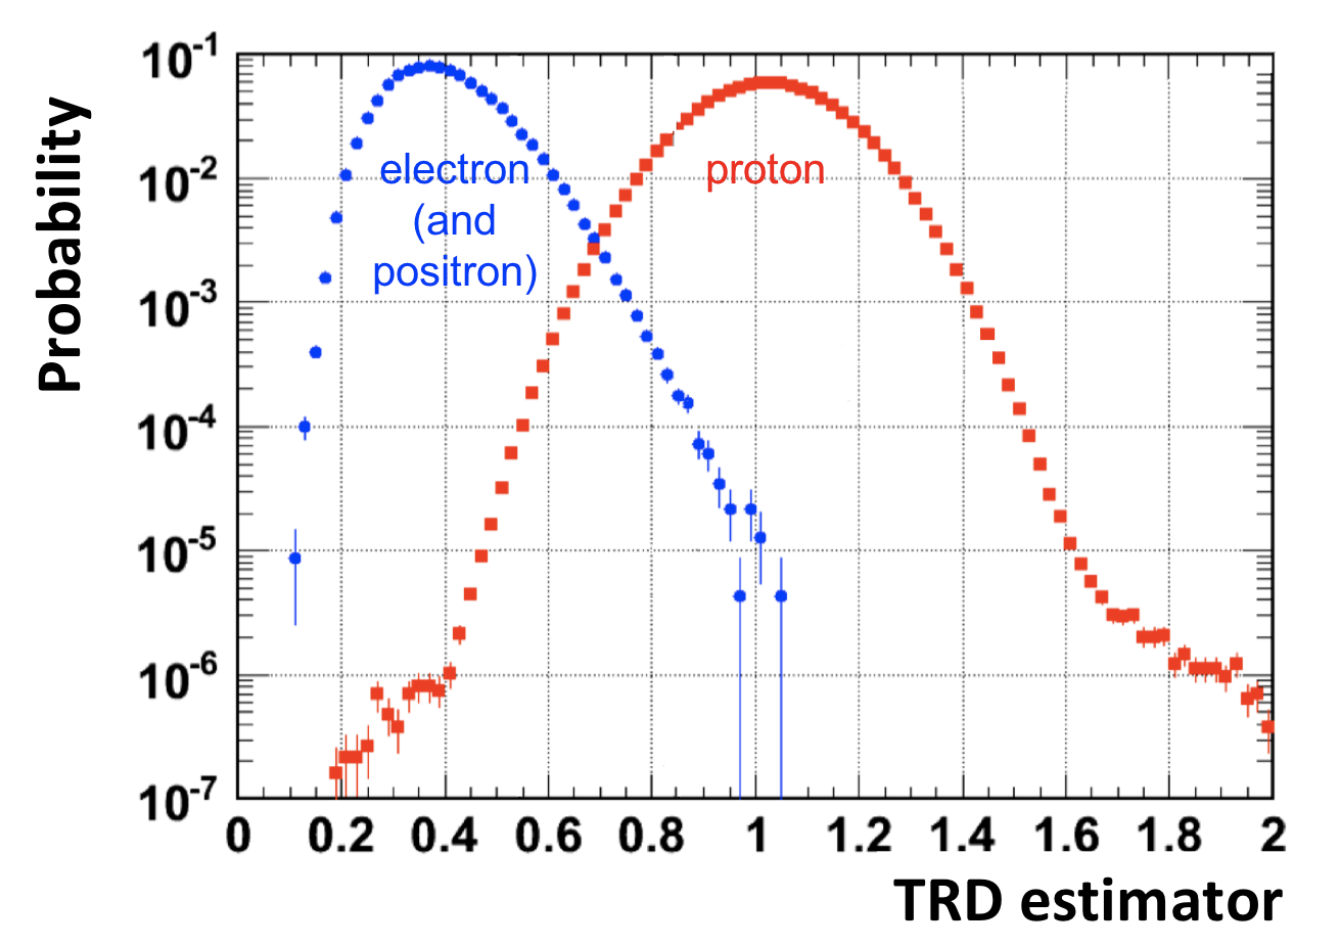
\includegraphics[width=0.80\textwidth]{Figures/chapter3/TRD/TRDEstimatorSeperation.png}
\includegraphics[width=1.00\textwidth]{Figures/chapter4/TRDLikelihood/{TRD_ChargeCorrectProtonTemplate_MC_B1042_pr.pl1.1800_7.6_all_Tree_positive_rigidity_14.1_15.3_pattern_0_bin_100_LogY_0.50}.pdf}
\caption[Seperation between the electrons and protons in $\Lambda_\mathrm{TRD}$ estimator.]{Seperation between the electrons and protons in $\Lambda_\mathrm{TRD}$ in the rigidity bin of 14.1 to 15.3 GV. The electrons and protons can be separated well in $\Lambda_\mathrm{TRD}$.}
\label{TRDEstimatorSeperation}
\end{figure}

the $\Lambda_\mathrm{TRD}$ provides separation power between electrons and protons. In figure \ref{TRDEstimatorSeperation}, the $\Lambda_\mathrm{TRD}$ is shown in the example rigidity bin of 14.1 to 15.3 GV, the electrons and protons can be distinguished well. At the 90\% electron efficiency range, the proton rejection power, which is defined as the inverse ratio of protons in this range, reaches more than $10^4$ \cite{TRDRejectionPowerPaper}. Similarly, the TRD likelihood estimator for the proton and the helium $\Lambda_{\mathrm{TRD}_{\mathrm{P/He}}}$ is defined as $-\rm{log}(\mathcal{L}_{p}/(\mathcal{L}_{p}+\mathcal{L}_{He}))$. \par


